\documentclass[../notes.tex]{subfiles}

\pagestyle{main}
\renewcommand{\chaptermark}[1]{\markboth{\chaptername\ \thechapter\ (#1)}{}}

\begin{document}




\chapter{Carbonyls}
\section{Problems 18 and 19}
\begin{itemize}
    \item \marginnote{9/11:}We should still continue reviewing the list of topics (at least before second year orals)!!
    \begin{itemize}
        \item I should also continue reading the textbook!!
        \item Come in with good solutions on Friday!!
    \end{itemize}
    \item Problem 22 is the \textbf{Dakin-West reaction}, if we want to look it up after class.
    \item We now begin discussing Problem 19.
    \begin{figure}[h!]
        \centering
        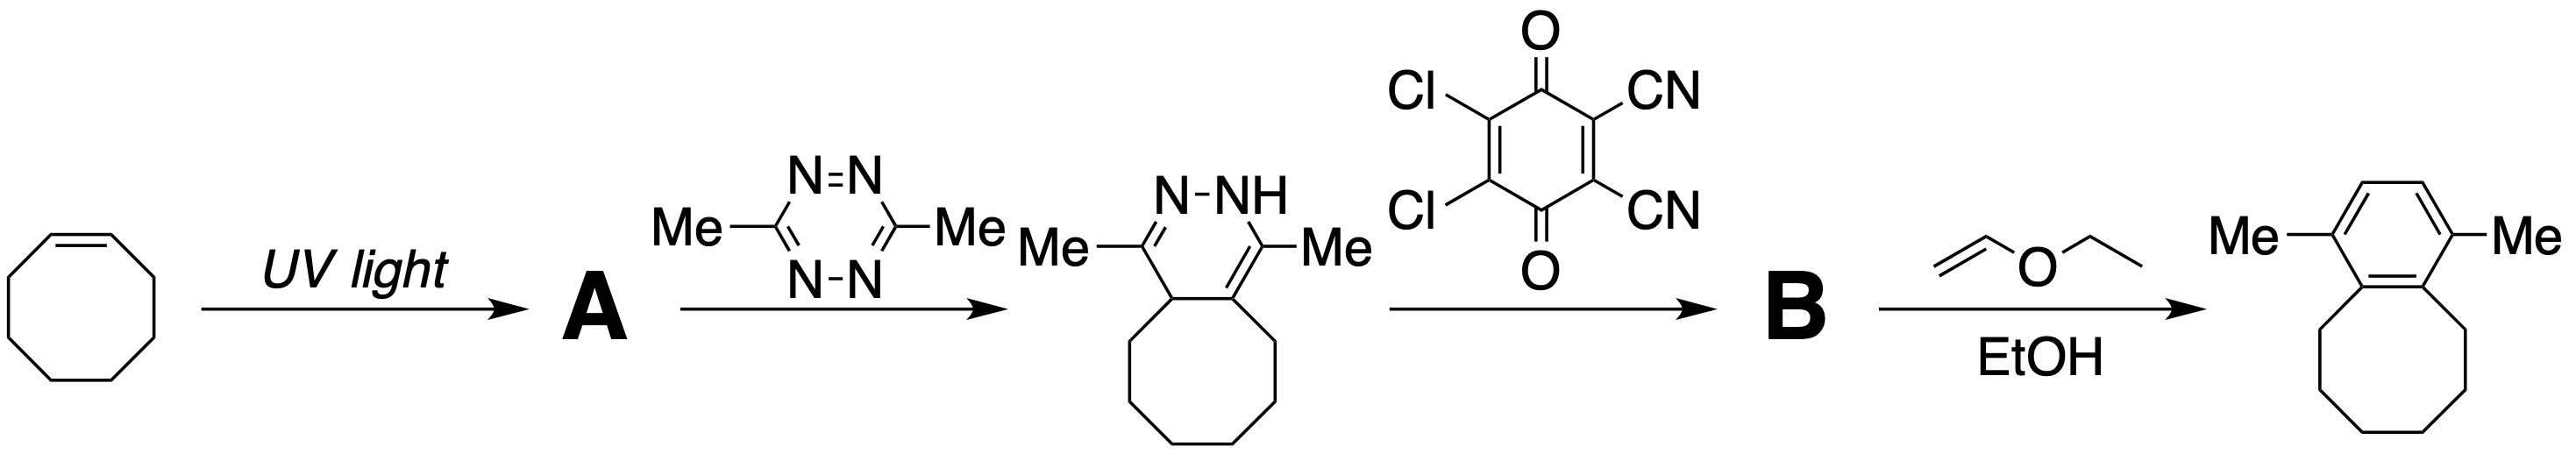
\includegraphics[width=0.9\linewidth]{JPSet1Q19.png}
        \caption{Johnson PSet 1, Q19.}
        \label{fig:JPSet1Q19}
    \end{figure}
    \item With UV light, we'll get isomerization to \emph{trans}-cyclooctene.
    \emph{picture; Frank's HOMO/LUMO diagram.}
    \begin{itemize}
        \item \emph{trans}-cyclooctene is a pretty strained molecule.
        \item Jeremiah has us draw out the HOMO and LUMO of the alkene, i.e., matching phases and unmatching phases.
        \item Jeremiah thinks the Woodward-Hoffmann rules are hard to understand without HOMO/LUMO diagrams.
        \item Light excites an electron to a higher energy state, in a process in which a spin is conserved.
        \begin{itemize}
            \item Learn \textbf{Jablonski diagrams}!!
            \item Absorption of a photon happens on a femtosecond timescale, way faster than any other process can happen.
            \item The flip of an electron spin is called \textbf{intersystem crossing}. This gets you from a singlet to a triplet state. ISC (flipping a spin) is technically a \textbf{forbidden} process, because a change in spin angular momentum must be matched by a change in orbital angular momentum or some such thing.
            \item The electrons are still paired, even after excitation.
            \item \textbf{Fluorescence} and \textbf{internal conversion} are by far the fastest and most favorable processes (photorelaxation and vibrational relaxation, respectively).
        \end{itemize}
        \item The double bond does break into a biradical, and now the molecule is much more conformationally flexible.
        \item Jeremiah likes to show a biradical as the unpaired electrons with their spins.
        \item What is the driving force for this thermodynamically uphill reaction?
        \begin{itemize}
            \item The \emph{trans} and \emph{cis} molecules absorb different wavelengths, so we need to shine exactly the wavelength that \emph{cis} can absorb so that the reaction doesn't go backwards.
            \item Once the \emph{trans} species forms, it will form in a 75:25 ratio or something like that because "the energy difference is matching the extinction coefficient" or something like that.
            \item Trans alkenes coordinate strongly to silver, and then we can flush it off of a silica column.
            \item The trans coordinates more to silver because...
        \end{itemize}
        \item An isolated double bond will need high intensity, low wavelength UV light be activated.
        \begin{itemize}
            \item If you wanted to get this to work with lower energy light, you'd need a photocatalyst.
            \item The reaction might start to have a bright color because the absorption peaks shift.
        \end{itemize}
    \end{itemize}
    \item The \emph{trans}-cyclooctene does a cycloaddition to form an intermediate.
    \begin{itemize}
        \item How do we do the proton shuffle? Perhaps using one of the nitrogens as a base.
        \item \textbf{Inverse electron demand Diels-Alder}. Here, the dieneophile is electron rich and the diene (a tetrazine) is electron poor.
        \begin{itemize}
            \item For this kind of reaction, we care about the LUMO of our diene and the HOMO of our dienophile (inverse of the regular Diels-Alder!).
            \item And we do see that the symmetry matches.
        \end{itemize}
    \end{itemize}
    \item Kicking out \ce{N2} and forming the double-bonded intermediate happens concerted; the zwitterion Frank drew probably doesn't exist.
    \item Then this intermediate tautomerizes to the intermediate in the question.
    \begin{itemize}
        \item Use an external molecule (or the solvent) to do the tautomerization. The second tautomer is more stable!
    \end{itemize}
    \item The third step is a \textbf{DDQ reaction}.
    \begin{itemize}
        \item There is no established mechanism for this reaction!
    \end{itemize}
    \item Net driving force: Taking two quinones and aromatizing both of them.
    \item It's also a dehydrogenation reaction.
    \item We believe the mechanism is radical-enabled.
    \item A $\pi$-bond (relatively nucleophilic) on the intermediate can do a single-electron transfer and become a radical cation.
    \begin{itemize}
        \item Single-electron transfer from a $\pi$-bond can and will happen if it's thermodynamically favorable because DDQ is such a good electron acceptor.
        \item You might also use light to accelerate this reaction.
    \end{itemize}
    \item There's a nice resonance structure that's aromatic, even though oxygen-centered radicals are unstable. But then this leads to rapid proton transfer of the resonance-stabilized positive proton.
    \item \textbf{Semiquinone} intermediate.
    \item Then the O radical steals an electron, becoming a negatively charged O that can steal a proton for aromaticity.
    \item There is also a proposed two-electron mechanism.
    \begin{itemize}
        \item Start with a hydride transfer of the most electron-rich hydride to DDQ.
        \item Using resonance structures to predict nucleophilic sites! Draw an aromatic resonance structure, which puts a positive charge on oxygen.
    \end{itemize}
    \item Why couldn't we use TEMPO to disprove the radical mechanism?
    \begin{itemize}
        \item It's a matter of relative rates; these radicals could only be formed transiently, far faster than TEMPO could interfere.
    \end{itemize}
    \item There are computational papers in the last few years on DDQ mechanisms, but they are heavily substrate dependent.
    \item Some calculations suggest an \textbf{asynchronous} process.
    \item There are some reactions that would almost definitvely suggest asynchronous mechanisms.
    \begin{itemize}
        \item SRN1 reaction fills the gaps where SN1 and SN2 don't work.
        \item Trigonal pyramidal carbocation is very unstable.
        \item Tertiary radical is much more simple.
        \item Doughtery and Ansyln has a whole chapter on SRN1 reactions!
        \item Prior to photoredox catalysis, these reactions were more just a curiosity; now we're trying to make them useful.
        \item Corey Stephenson's work on the early photoredox reactions.
    \end{itemize}
    \item Lastly, we get another Diels-Alder reaction followed by a retro-Diels-Alder to kick out \ce{N2}.
    \item Then six-membered transition state proton transfer.
    \begin{itemize}
        \item Heat or acid would help the end.
        \item Jeremiah ran this reaction when he first got to MIT, and thought that the spontaneous aromatization was quite interesting.
    \end{itemize}
    \item Altogether, the full solution to PSet 1, Q19 is on the next page.
    \pagebreak
    \item We now begin discussing Problem 18.
    \begin{figure}[h!]
        \centering
        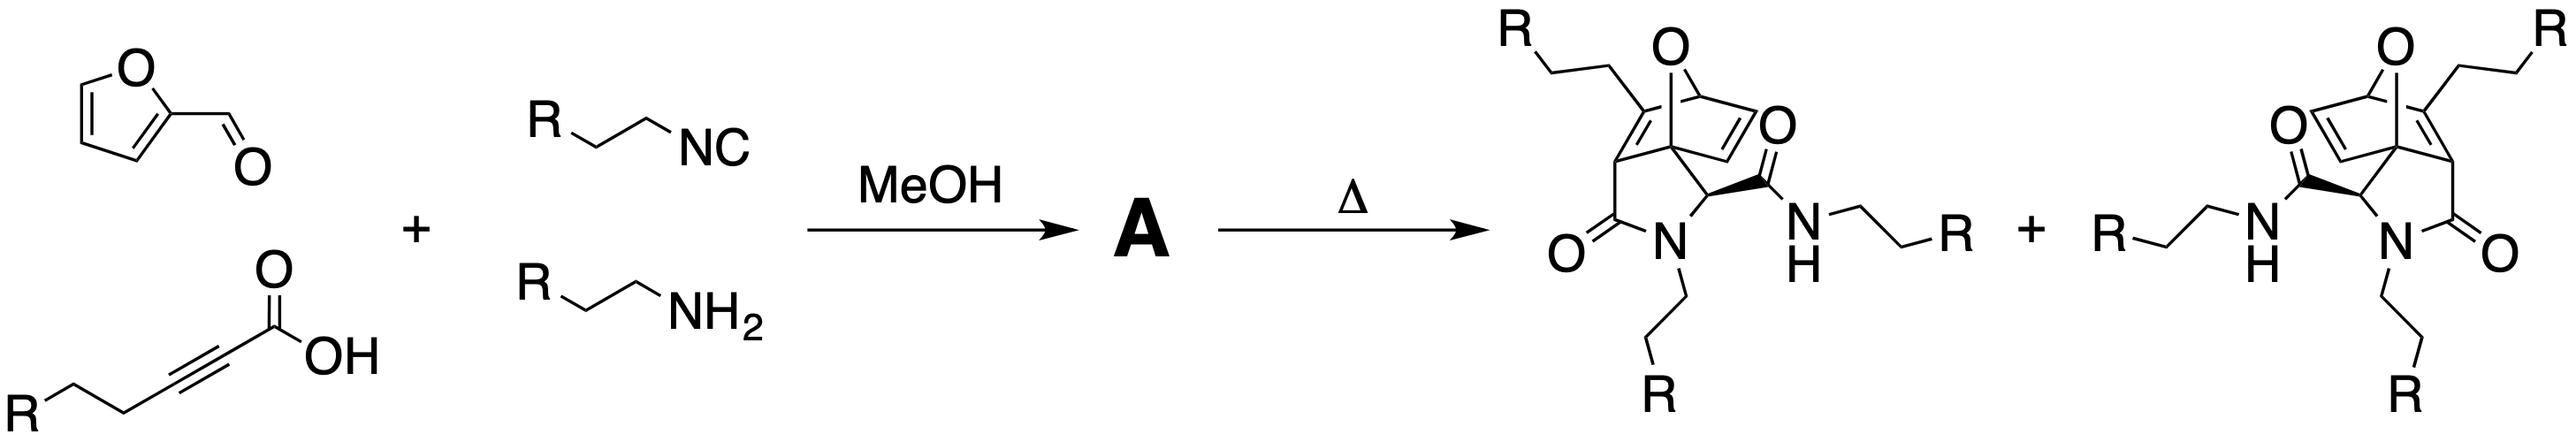
\includegraphics[width=0.9\linewidth]{JPSet1Q18.png}
        \caption{Johnson PSet 1, Q18.}
        \label{fig:JPSet1Q18}
    \end{figure}
    \item Altogether, the full solution to PSet 1, Q18 is on the next page.
    \begin{figure}[h!]
        \centering
        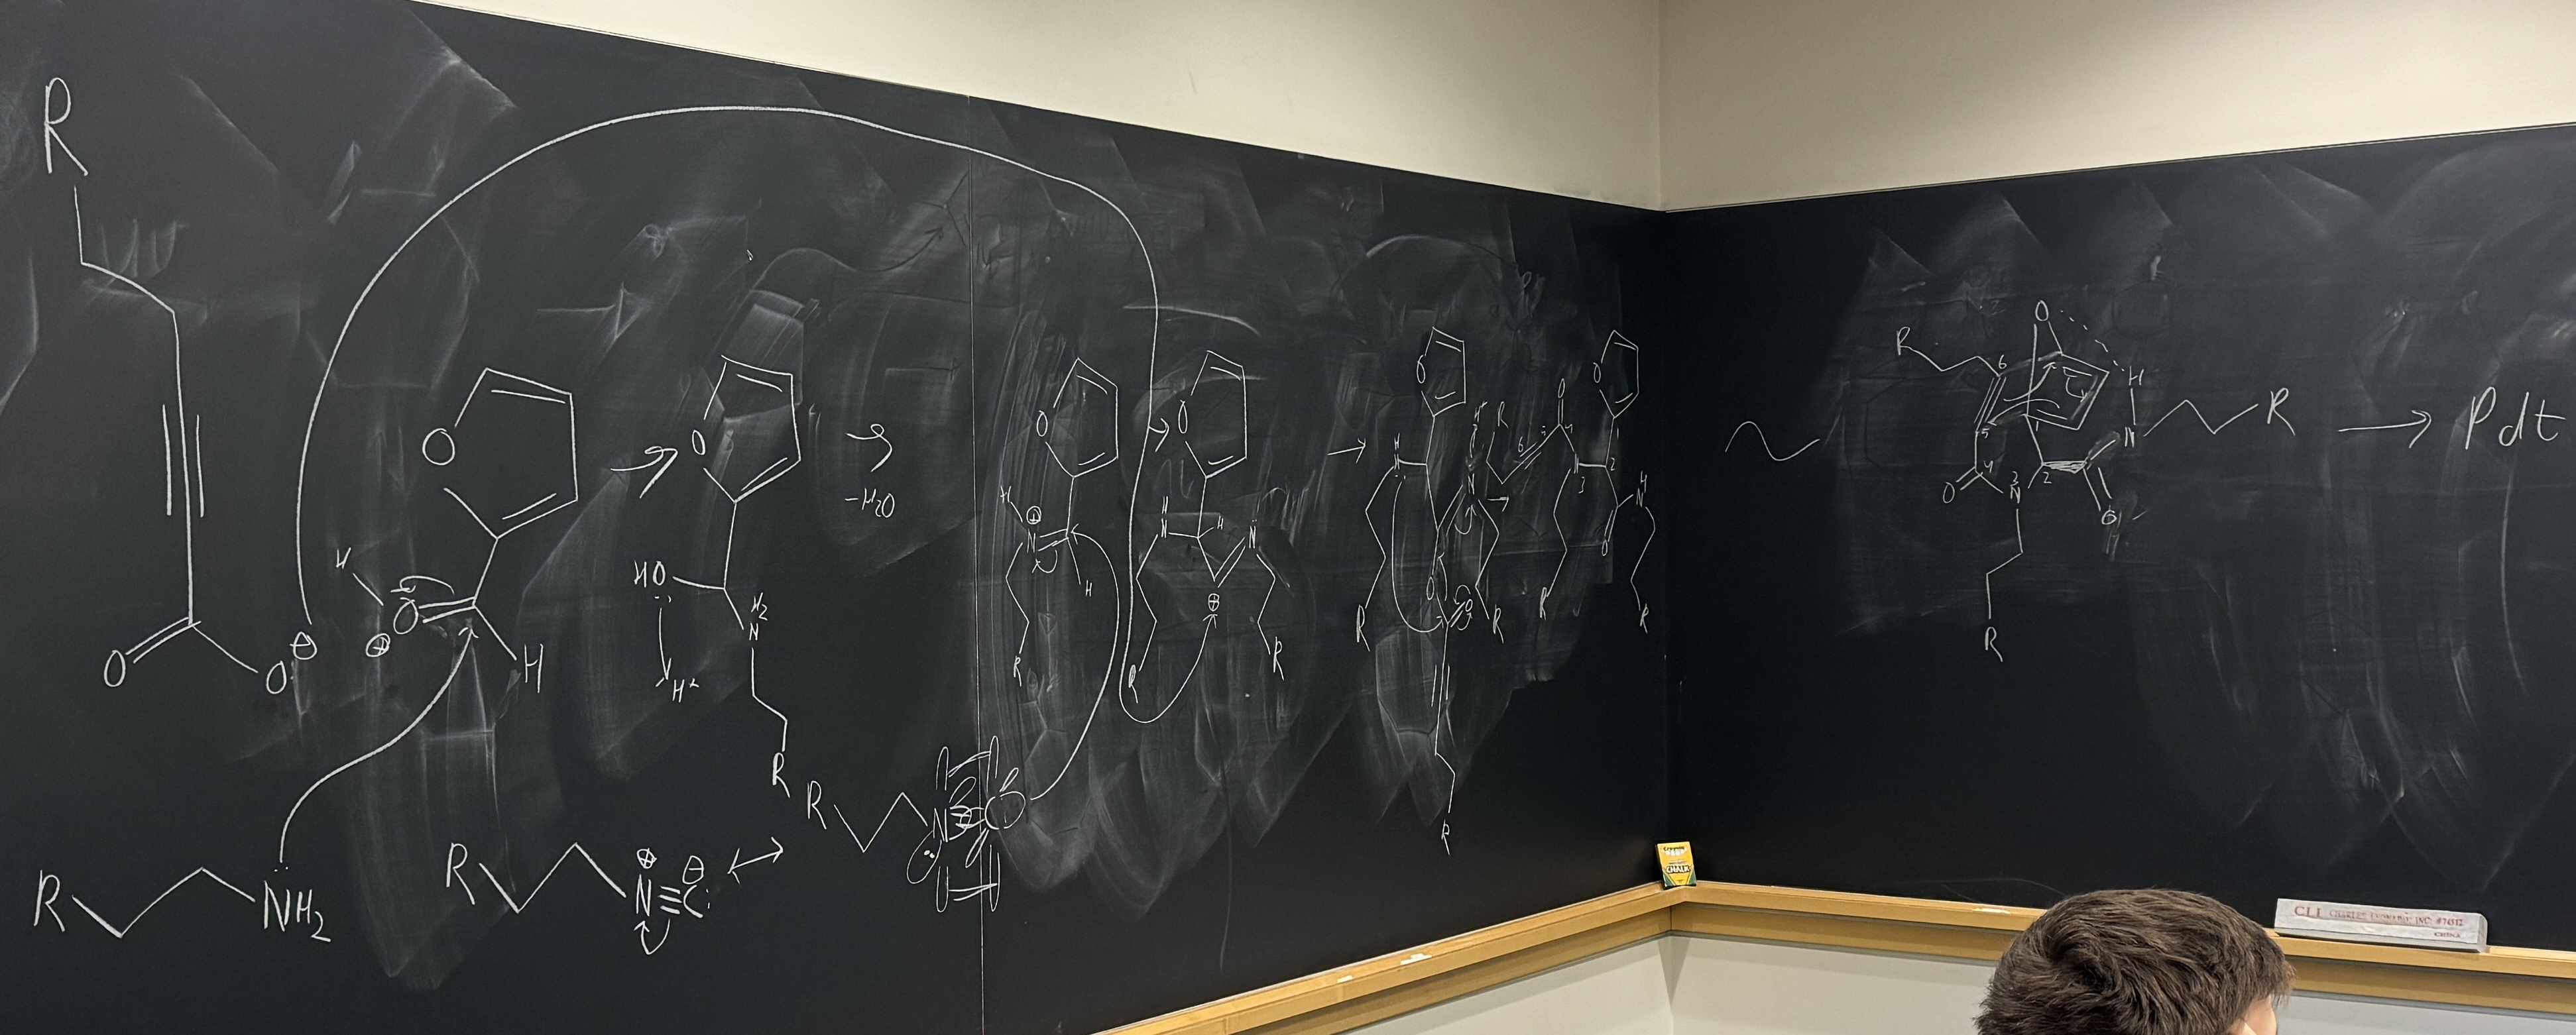
\includegraphics[width=0.8\linewidth]{JPSet1Q18S.JPG}
        \caption{Johnson PSet 1, Q18 solution.}
        \label{fig:JPSet2Q18S}
    \end{figure}
    \pagebreak
    \item We now begin discussing Problem 21.
    \item The first step is a \textbf{Fischer indole synthesis}.
    \item That's all we got to today.
    \item Jeremiah's list of named reactions.
    \begin{itemize}
        \item 15: Benzoin condensation reaction.
        \item 18: Ugi reaction followed by Diels-Alder.
        \item 19: Inverse electron-demand Diels-Alder and another Diels-Alder.
        \item 20: A Michael addition and Mannich reaction.
        \item 22: A Dakin-West.
        \item 21: Fischer indole synthesis.
    \end{itemize}
\end{itemize}




\end{document}